\section{Evaluation}
\label{sec:evaluation}

We have implemented metadata persistence on the latest version of
DM-Cache running on Linux kernel version 3.3. To evaluate this we use
the workloads offered by the IOZone benchmark to evaluate the overhead
of this mechanism.

For testing we connected two machines via iSCSI. One machine serves as
the iSCSI-target/network-storage and is running Ubuntu 11.10. The
second machine serves as the iSCSI-client running Arch Linux with the
3.3 kernel and issues the storage requests to the iSCSI-target.

We evaluated our approach on an Mtron Pro 7500 64GB SSD. We used an
Mtron SSD to get a good upper bound on our performance overhead as
Mtron SSD's (as compared to Intel and Vertex SSD's) have slower write
performance \cite{FIOS}.

Due to issues with the implementation of the write-back mechanism
within DM-Cache we only show evaluation of DM-Cache using our
persistence mechanism with write-through. Our testing shows no issues
with the actual data when running experiments but the kernel logs show
some file-system warnings so we omit those results.

\subsection{IOZone}

We use the IOZone benchmark to evaluate the throughput of DM-Cache as
a cold cache with and without metadata persistence enabled as well as
a warm cache with and without metadata persistence enabled to
calculate the overhead.

Because we are only using the write-through mechanism in our
evaluation the only throughput results that are meaningful to us are
the read throughput statistics. Reread is not significant because that
will use the data that is cached in RAM.

For each test run we create and initialize a new cache and run IOZone
on different sized caches and record the results. We use cache sizes
of 512MB, 1GB and 2GB. To evaluate the results of a warm cache we
simply run the read workload in IOZone and then drop the page cache
for the system so that it is forced to do I/O rather than simply
reading the information from RAM while the information is still stored
in the cache.

\graphicspath{{../Results/}}

\begin{figure}[t]
  \caption{IOZone Read Workload with Cold Cache}
  \centering 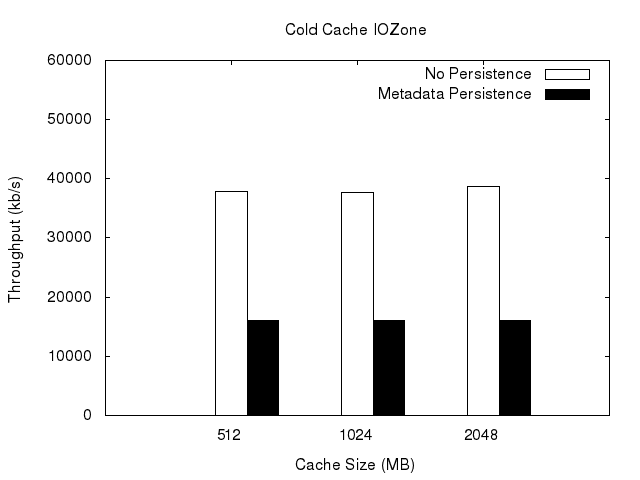
\includegraphics[width=0.5\textwidth]{results_first.png}
  \label{fig:iozone-cold}
\end{figure}

\begin{figure}[t]
  \caption{IOZone Read Workload with Warm Cache}
  \centering 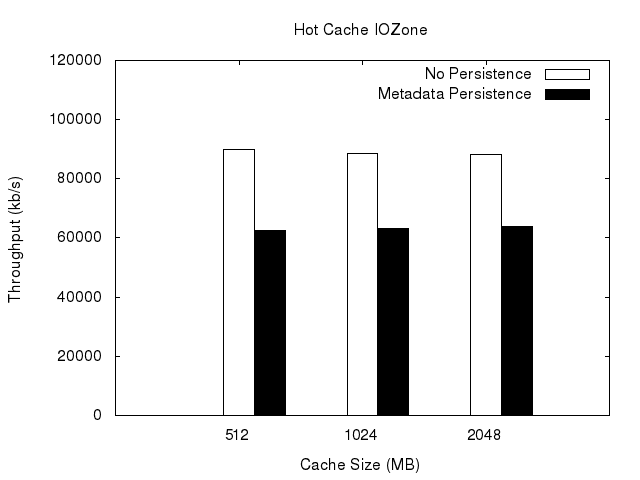
\includegraphics[width=0.5\textwidth]{results_second.png}
  \label{fig:iozone-warm}
\end{figure}

In Figure~\ref{fig:iozone-cold} it can be seen that inserting a lot of
blocks into the cache along with our metadata persistence mechanism
causing extra writes can slow down performance by about 50\%. This is
because metadata is being updated constantly because every block
fetched is not cached so it has to be written to the cache device
along with relevant metadata for each
block. Figure~\ref{fig:iozone-warm} shows that once the cache has
reached a state where access is mostly read hits performance comes
closer to a cache without persistence by about 75\%.
